\documentclass[conference]{IEEEtran}
\usepackage{graphicx}

% correct bad hyphenation here
\hyphenation{op-tical net-works semi-conduc-tor}


\begin{document}
%
% paper title
% can use linebreaks \\ within to get better formatting as desired
\title{Suboptimal Time management in Non-ideal Shared space}


% author names and affiliations
% use a multiple column layout for up to three different
% affiliations
\author{\IEEEauthorblockN{Praveen Kumar Pendyala}
\IEEEauthorblockA{Information and Communication Engineering\\
Technische Universitat Darmstadt\\
Email: m@praveen.xyz}}

% make the title area
\maketitle


\begin{abstract}
%\boldmath
Time management is an asset and a liability. Lack of proper time management may put oneself on a depression feedback loop [1]. Time management is a melange of various aspects - scheduling tasks, execution and time line corrections, to name a few. Each of these aspects can be thought as a subproblem in our attempts to tackle the grand problem - Optimal Time Management. In addition to these subproblems, we must accept the fact that we live in a non-ideal world along with many others - shared space.  The paper deducts the need for adaptive, suboptimal Time Management techniques while taking external stimuli into consideration.
\end{abstract}


% For peer review papers, you can put extra information on the cover
% page as needed:
% \ifCLASSOPTIONpeerreview
% \begin{center} \bfseries EDICS Category: 3-BBND \end{center}
% \fi
%
% For peerreview papers, this IEEEtran command inserts a page break and
% creates the second title. It will be ignored for other modes.
\IEEEpeerreviewmaketitle


\section{Introduction}
% \IEEEPARstart
Time and Time Management are of paramount importance. This brings in an obvious urge to develop various techniques for an optimal time management technique - starting from marking calenders to a rigid time plan accounting for each hour of a day. There are a whole lot of techniques to make a basic plan, some of which will be covered in the existing literature section. One major aspect of time management is making a perfect schedule but an even more crucial step concerns with the execution. There are several factors that could keep one from meeting their time plan. Stress, Bad planning, Lack of self control and so on so forth.

The source of all the factors that affect time plans, broadly speaking, are a result of the fact that we live in a shared space where we are affected not only by our own actions but also by the choices of those around us, and that we live in a non-ideal world where most events are probability based, not guided by any standard Uncertainty Principle, thus bringing in more players into the equation. All these complex parameters would push any purely mathematical or conceptual approach to derive an optimal time plan into solving an NP-Hard problem [2]. One has to live with a suboptimal time plan for a given situation, iterate it based on their needs and arrive at an acceptable compromise between an ideal and a executable plan.

The following contents of the paper are divided into four sections. Section II - Existing literature, would focus on some of the existing techniques for Time management. Followed by Section III - Identifying factors, where we identify a list of factors that could affect ones time plan and identify plausible ways to workaround them. Section IV - Execution and Evaluation, which is completely spanned by a case study where the subject employs an adaptive time management technique for their day to day activity for two fortnights and we would discuss the outcomes of the experiment in light of the existing and proposed theory. We will then conclude with Section V - Conclusions, where we would be highlighting the key aspects of our argument and how it compared to our observations in the case of our test subject.

\section{Existing literature}
There is plethora of research related to Time Management (TM) techniques and surveys depicting the outcomes of adopting or otherwise of a TM technique. [3], [4] and [5] centered their work around the impact of TM in an academic context, backing their claims through surveys with varying size of sample space and interpretations but similar outcomes. [6], in contrary to the above mentioned research, suggests that Time Management behaviors may have beneficial effects on tensions and job satisfaction but not on job performance and contrary to popular claims, time management training was not found to be effective. This also controverts the hypothesis and findings of [7] and [8]. There is plenty of existing and ongoing research related to the identification of the nature and magnitude of the affects Time management has on its subjects but, it is beyond the scope of this paper. The references mentioned above could be a good starting points for gaining different, possibly contradictory, perspectives at the issue.

\begin{figure}[hb]
  \centering
  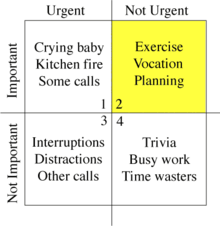
\includegraphics[width=2.8in]{eisenhower}
  \caption[]
   {A basic "Eisenhower box" to help evaluate urgency and importance.}
\end{figure}

Some of the common time management methodologies are Pareto analysis, ABC analysis, The Eisenhower Method and POSEC method. The central idea of Pareto analysis is that 80\% of tasks can be completed in 20\% of the disposable time - The 80-20-rule to increase productivity [12]. ABC analysis is often used in business management for categorization of large data into groups [11]. These groups are often marked as follows:
\begin{itemize}
  \item A -- Tasks that are perceived as being urgent and important
  \item B -- Tasks that are important but not urgent
  \item C -- Tasks that are neither urgent nor important
\end{itemize}
Each group is then rank-ordered by priority. On the other hand, The Eisenhower Method uses the Eisenhower Decision Principle through which, all tasks are evaluated using the criteria important/unimportant and urgent/not urgent, and then placed in according quadrants in an Eisenhower Matrix as shown in figure 1. Last in our list, POSEC method is an acronym for Prioritize by Organizing, Streamlining, Economizing and Contributing. Inherent in the acronym is a hierarchy or priority of task ordering:
\begin{enumerate}
  \item \textbf{P}rioritize -- Define your time and your goals.
  \item \textbf{O}rganize -- Things you have to accomplish regularly to be successful. Examples include family and finances.
  \item \textbf{S}treamline -- Things you may not like to do, but must do anyway due to existing constraints. Examples include work and chores.
  \item \textbf{E}conomize] -- Things you should do or may even like to do, but they're not pressingly urgent. Examples include pastimes and socializing.
  \item \textbf{C}ontribute -- By paying attention to the few remaining things that make a difference. Examples include social obligations.
\end{enumerate}
There are also time management approaches that emphasize the need for more focused and simple implementation, including the approach of "Going with the Flow" - natural rhythms, Eastern philosophy.


All the methods we discussed earlier are theoretical constructs which suggest various ways we could opt to manage time or tasks. Since we live in a digital world, it is a natural tendency to seek computer-aided tools - Desktop, Smart phone or Web applications, that can help follow a schedule of choice in a more convenient fashion. There are in fact many software tools that have already integrated one or more of the above techniques and available on the App stores. However, only a small portion of them are actually developed out of independent academic research. These computer-aided task or time tracking tools are often a good way for tracking or analyzing the time plans and also simplifies the job of identifying the short comings. Many companies use time tracking software to track an employee's working time, billable hours etc.,. [14] is one such multi purpose tools which, in addition to location tracking, also offers activity logging and tagging. This actually leads to a better contextual information on the activity and its progress.

The common shortcoming in all these literatures is their failure to account that test subjects could be influenced by a plethora of external and internal factors. All these influencing factors, broadly speaking, are a result of Non-idealistic behavior and shortcomings of the test subjects and negative, intended or unintended, influence from peers, colleagues and other indirect players on test subject's attempts in keeping up with their schedule. Attempts have been made to evaluate the extent of influence by a common factor, tendency of procrastination, on the effective execution of ones time plan [9], [10].


\section{Identifying factors}
There are a plethora of factors that could disrupt a time plan and they can be broadly categorized into External and Internal factors. Internal factors are those that solely dependent on the individual or arise as an outcome to an individuals actions. While External factors are the ones which the individual may not have anticipated or predicted at the time of planning and mostly a result of the actions of external entities.

\textbf{Internal factors:} Some common examples of Internal factors are Stress, Bad planning, Lack of self control and Addictions, all of which are outcomes of a person's own shortcomings. These are the ones which are entirely under the control of the individual - attempting to follow a routine, alone. More often than not, these factors can be corrected by having a greater perseverance, self control and dedication on the part of the person following or trying to follow a routine. Some of the other tricks that could work is developing habits out of the plan - Motivation is what gets them started while habit is what keeps them going.

\textbf{External factors:} These on the other hand, cannot be controlled by the individual alone. Most commonly, external factors occur as a consequence, either direct or indirect; deliberate or unintentional, actions of those around the subject. Due to the very nature of the cause of these factors, the countermeasures are not as uncomplicated as that of the Internal factors. Often times they are hard to prevent within the control of the subject. So, the next best and feasible approach to tackling External factors is to employ appropriate degree of flexibility in the time plans to alleviate the possible damage. Identifying the source of these factors could often assist in estimating a suitable level of flexibility that should be incorporated into the plan. Other alternatives include iterative time line corrections or adjustments to meet the new constraints or shortcomings.


\section{Execution and Evaluation}
We analyzed the day-to-day life executions of a test subject and how they divulge from their expected time plan. A qualitative note on the external factors causing the time-line diversion is also provided corresponding to each diversion.


\begin{figure}[hb]
  \centering
  \renewcommand{\arraystretch}{2}
	  \begin{tabular}{ | l | c | }
		\hline
		\textbf{Activity type} 	& \textbf{Time spent per day} 	\\ \hline
		Sleep					& 	8 Hours						\\ \hline
		Job						& 	5 Hours						\\ \hline
		Lectures				& 	3 Hours						\\ \hline
		Learning				& 	3 Hours						\\ \hline
		Leisure					& 	5 Hours						\\ \hline
	  \end{tabular}
  \caption[]
   {Static reference time line plan made by the test subject}
\end{figure}

We began the experiment by making a static time plan for the test subject as shown in figure 2. This serves as a reference while the actual time spent on a given activity per day, almost always, is different from the planned schedule. The differences are mostly consistent over span of few days which tells us that the external factors causing this offset are stable influences coming from the shared space concept depicted earlier. To shed some more light on this behavior, we calculated the time spent per activity in a period of one week and tabulated the values for four weeks as shown in figure 3. 

\begin{figure}[hb]
  \centering
  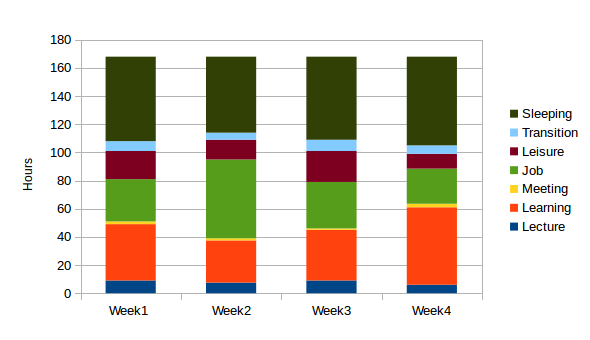
\includegraphics[width=3.7in,height=3.0in]{bar}
  \caption[]
   {Hours spent per activity in a week for a period of four weeks}
\end{figure}

An interesting observation here is that, only a certain type of activity times vary significantly across weeks while others are nearly stable. The relatively stable time share is taken on every week by Sleep, Transition and Lectures. The significantly varying ones are Leisure, Job and Learning. There are plenty of reasons and factors for these digressions. We can qualitatively identify a subset of the factors causing these deviations in a given week compared to the average or planned static time line. While doing so, we shall also identify the category of the factor - external or internal, that resulted in the change. 

The factors that influence an increased shared in Job activity are mostly external. Some of these factors include, but not limited to, work related deadlines, presentations and goals. The ones that root for a share increase of Academic activities - Learning and Lectures are also external. And the major factors in this list are Lab work, Lab demos, Exams and other academic deadlines. We can also notice a dip in Lectures timeshare in week 4 where the subject is loaded by other forms of academic activity like project or lab deadlines. This change, broadly speaking, is a result of external factors and another interesting phenomena to notice here is that it is also a result of constrained total time for the sum of activity times in a category.


\begin{figure}[hb]
  \centering
  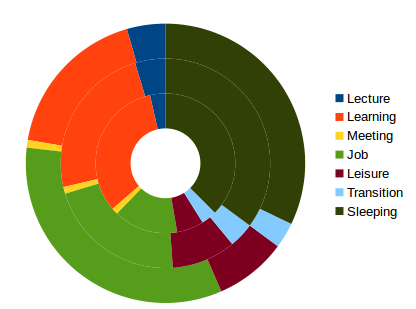
\includegraphics[width=3.7in]{donut}
  \caption[]
   {Concentric rings pie chart depicting the time share of each activity in a week over 3 different week samples. Innermost ring represents learning dominated week, middle ring for average over four weeks, outermost ring represents job dominated week}
\end{figure}

The variance in activity time share can be observed better in figure 4. where we identified two extreme weeks - one involving a greater share on Academic activity and the later with a greater share on Work activity, and compared it with an average time share of each activity over the whole period of four weeks. The notion of the rings is as follows:
\begin{itemize}
  \item Innermost ring -- represents learning dominated week
  \item Middle ring -- for average over four weeks
  \item Outermost ring -- represents job dominated week
\end{itemize}
The arc angle covered by the stable activities is nearly same across all the rings while the unstable activities showing an angular variance of 10-15 percent. The not so high, yet not negligible, variance in dynamic activity timeshares indicate that the concept of a single static reference is bad and good at the same time. This leads us to believe that influences from external factors are inevitable and test subject has employed subjective ways to cope up with them and follow a suboptimal time management scheme. The stable arcs -- Sleep, Transition and Lectures are the ones that are more likely to be affected only by internal factors. As we discussed earlier, the internal factors can be overcome by developing habit and exhibiting a greater control. The varying arcs -- Leisure, Job and Learning, on the other hand have mutual dependencies - since the total time in a given day is constant, and are susceptible to change by External factors like work related deadlines, presentations, team work and group goals. Since some of these factors are primarily dependent on group outcomes, they are prone to changes and are often hard to workaround unless everyone else agrees to be on the same page and cope up to the same pace. Although getting everyone in a team on the same page is a possible and often implemented norm, pace is very subjective - not just to a person but also to their psychological state at a point in time. These are one of the reasons why external factors are hard to deal with and cannot be addressed through prevention strategies. What works and in fact implemented by the test subject is employing appropriate damage mitigation strategy to deal, as and when a disturbance did occur due to one of the external factors. 


\section{Conclusions}
We presented the existing literature on Time management, majority of which dealt with assumptions of static time management. We then followed on to listing factors - external and internal, that affect such a scheme and established the need for adaptive or dynamic planning. We presented a case study on Test subject who employed a static time plan to start with and displayed significant deviations from the plan on day-to-day basis. We observed patterns in this deviations and provided a qualitative analysis of plausible external factors that may have caused the deviations for each type of activity over one week. We have also covered the ways in which one could overcome Internal factors - mostly by developing habits and having perseverance, and External factors - by allowing room for time line changes or iterate modifications to time plan. 

In conclusion, we established that we are affected by various factors in following a static time line and that majority of these stimulus are a direct implication of the fact that we live in a non-ideal world of probabilities along with others. Thus one may employ a static time plan which may be used as a reference and should be willing to adapt to the changes.

% use section* for acknowledgement
\section*{Acknowledgment}
The author would like to extend his gratitude to the Telecooperation Group of TU Darmstadt for providing the required tools and resources, which form the basis for Test Subject Data collection and served as seed for this paper.


% trigger a \newpage just before the given reference
% number - used to balance the columns on the last page
% adjust value as needed - may need to be readjusted if
% the document is modified later
%\IEEEtriggeratref{8}
% The "triggered" command can be changed if desired:
%\IEEEtriggercmd{\enlargethispage{-5in}}

% references section

\begin{thebibliography}{1}

\bibitem{IEEEhowto:}
\emph{Yoga Journal}, \relax May-Jun 1976, pp. 17.

\bibitem{IEEEhowto:}
Aaronson, Scott. \emph{"NP-complete problems and physical reality."} ACM Sigact News 36.1, 2005, pp. 30-52.

\bibitem{IEEEhowto:}
Britton, Bruce K., and Abraham Tesser. \emph{"Effects of time-management practices on college grades."} Journal of educational psychology 83.3 (1991): 405.

\bibitem{IEEEhowto:}
Macan, Therese H., et al. \emph{"College students' time management: Correlations with academic performance and stress."} Journal of educational psychology 82.4 (1990): 760.

\bibitem{IEEEhowto:}
Misra, Ranjita, and Michelle McKean. \emph{"College Students' Academic stress and its relation to their Anxiety, Time Management, and Leisure satisfaction."} American Journal of Health Studies 16.1 (2000): 41-51.

\bibitem{IEEEhowto:}
Macan, Therese Hoff. \emph{"Time management: Test of a process model."} Journal of applied psychology 79.3 (1994): 381.

\bibitem{IEEEhowto:}
Adams, Gary A., and Steve M. Jex. \emph{"Relationships between time management, control, work–family conflict, and strain."} Journal of Occupational Health Psychology 4.1 (1999): 72.

\bibitem{IEEEhowto:}
Waterworth, Susan. \emph{"Time management strategies in nursing practice."} Journal of Advanced Nursing 43.5 (2003): 432-440.

\bibitem{IEEEhowto:}
Lay, Clarry H., and Henri C. Schouwenburg. \emph{"Trait procrastination, time management, and academic behavior."} Journal of Social Behavior and Personality (1993).

\bibitem{IEEEhowto:}
Gafni, Ruti, and Nitza Geri. \emph{"Time management: Procrastination tendency in individual and collaborative tasks."} Interdisciplinary Journal of Information, Knowledge, and Management 5 (2010): 115-125.

\bibitem{IEEEhowto:}
Lakein, Alan. How to Get Control of Your Time and Your Life. New York: P.H. Wyden (1973)

\bibitem{IEEEhowto:}
Timothy Ferris. \emph{"The 4-Hour Workweek."} Crown Publishing Group (2007)

\bibitem{IEEEhowto:}
McKay, Brett and Kate. \emph{"The Eisenhower Decision Matrix: How to Distinguish Between Urgent and Important Tasks and Make Real Progress in Your Life."} A Man's Life, Personal Development. (October 23, 2013)

\bibitem{IEEEhowto:}
Schweizer, Immanuel, and Benedikt Schmidt. \emph{"Kraken. me: multi device	 user tracking suite."} Proceedings of the 2014 ACM International	Joint Conference on Pervasive	and	Ubiquitous Computing: Adjunct Publication. ACM, 2014.


\end{thebibliography}




% that's all folks
\end{document}


